\chapter{Unsupervsed Learning}
\label{ch:Unsupervised}

In the previous \autoref{ch:MachineLearning}, an overview of the most common supervised learning algorithms has been provided, but all these techniques require a labeled dataset. As anticipated in the introduction, most of the time a model of the machine to be monitored is not available. Furthermore, usually a prior knowledge of the behavior of the machine in the \emph{healthy} or a \emph{faulty} state is not available either. Even in the best case scenario, where some data collection has been done, the data will be unlabeled. 

To address this scenario, two approaches are possible: either label the data, or use an unsupervised learning algorithm. The former would be tedious and time-consuming in the case the dataset contains both healthy and faulty data, because the faulty data would have to be labeled by hand. If the dataset contains only healthy data, it would be trivial to automatically label all the instances as healthy and use a supervised learning algorithm, but this would be a stretch of the definition of supervised learning. The latter is a more linear approach, since unsupervised learning algorithms are designed to work with unlabeled data.

The most common unsupervised task is dimensionality reduction \citepage{hands-on-geron2022}{260} but, in this thesis, the main focus will be on novelty detection, fault detection and predictive maintenance, so the considered \gls{uml} algorithms will be clustering and density estimation.

\paragraph[]{Clustering}
Clustering is the task of grouping together similar instances. The definition of \emph{similar} depends on the algorithm used. The most common algorithms are {k-means} and \gls{dbscan}. The former is a \gls{glo:cent}-based algorithm, it is fast to evaluate a new instance and produce a lightweight model but performs poorly in some conditions that will be described in detail. The latter is a density-based algorithm, it performs better in the condition where k-means fails, but has the drawbacks of being much slower to evaluate a new instance, and to perform novelty detection, the proposed solution has to keep all the train data in memory. Both will be described in detail in the following \autoref{sec:kmeans} and \autoref{sec:dbscan}.

\paragraph[]{Gaussian mixture models}
The second approach to novelty detection is the use of Gaussian Mixture Models (\gls{gmm}). This approach is based on the assumption that the data is generated from a mixture of several Gaussian distributions with unknown parameters \citepage{hands-on-geron2022}{283}. Then the distribution model can be used for novelty detection. This approach will be described in detail in the following \autoref{sec:gaussian}.

\paragraph{Other approaches}
At the end of the chapter, some other approaches will be briefly described and tested on the same dataset used for demonstrating clustering and \gls{gmm}. These approaches are: \gls{iforest}, \gls{lof} and $\nu$-\gls{svm}. The first two are based on the assumption that outliers are instances that are isolated from the rest of the data, while the latter is based on a kernelized \gls{svm} algorithm. 

\section{K-means}
\label{sec:kmeans}

This problem is called k-means because it aims to describe the \quoted{clustering} by separating the data into \gls{glo:clust}s ($\gls{sym:cluster}$), and define each cluster with its mean ($\gls{sym:cent}$). Note that the mean of the cluster, from a physical point of view, is the center of mass of the cluster itself as if it is composed of unitary point masses located at the positions of the datapoints. The mean is not necessarily a point belonging to the cluster.

Let's assume to have extrapolated $F$ features from each of our signals, to produce a set $\gls{sym:snapset}$ of $n$ {\gls{glo:snap}}s $\gls{sym:snap}_i, i \in [1,n], \gls{sym:snap}_i \in \gls{sym:snapset} $ (every {\gls{glo:snap}} is a vector of features $\in \mathbb{R}^F$). The task is to define a set $\gls{sym:cluster}$ of $k$ clusters ($k \leq n$) $\gls{sym:cluster}_i, i \in [1,k], \gls{sym:cluster}_i \in \gls{sym:cluster}$ that minimize the squared sum of the distances between the {\gls{glo:snap}}s and the {\gls{glo:cent}}s $\gls{sym:cent}_i$ of the clusters they belong to. This is equivalent to finding the {\gls{glo:cent}}s that minimize the \textbf{variance} of the clusters themselves, so the problem can be formulated as in the \autoref{eq:kmeans_problem}.

\begin{equation}
  \argmin{\gls{sym:cluster}}\sum_{i=1}^{k}\sum_{\gls{sym:snap}_j \in \gls{sym:cluster}_i} \norm{\gls{sym:snap}_j - \gls{sym:cent}_i}^2 = \argmin{\gls{sym:cluster}}\sum_{i=1}^{k}\abs{\gls{sym:cluster}_i}\mathrm{Var}\gls{sym:cluster}_i
  \label{eq:kmeans_problem}
\end{equation}

Unfortunately, this problem is NP-hard, even for as little as $F=2$ features considered \cite{MAHAJAN201213}, so it is not possible to guarantee finding the global optimum in a reasonable time.

Anyway, {\gls{glo:heuristic}} clustering algorithms were already developed in the 1950s. 
The first appearance of the term \quoted{K-means} was used in 1957 by MacQueen \cite{macqueen1967some}, and the algorithm settled to a \quoted{standard} version, published by Stuart Lloyd in 1982 \cite{Lloyd1982} (but developed at Bell Labs in 1957).

Among all the unsupervised clustering algorithms, a survey from 2002 \cite{berkhin2002survey} stated that K-means \quoted{is by far the most popular clustering algorithm used in scientific and industrial applications}. A more recent survey from 2019 \cite{Abla2019survey}, cited this algorithm as first in the group of four most popular algorithms.

Nowadays, the K-means algorithm is implemented in many libraries, such as \texttt{scikit-learn} for \texttt{Python}, and others for \texttt{C}, \texttt{R}, \texttt{MATLAB}, etc. However, the runtime performances vary widely depending on the implementation \cite{Kmeans-performances-Kriegel2017}. The problem of the algorithm returning a local minima instead of the global one is still present. Most implementations try to minimize the probability of returning this sub-optimal result by running the algorithm multiple times with different initializations and then selecting the best result, so the problem of getting a sub-optimal result is not a common issue in practice.

\subsection{Training}

\begin{figure}[htbp]
  \centering
  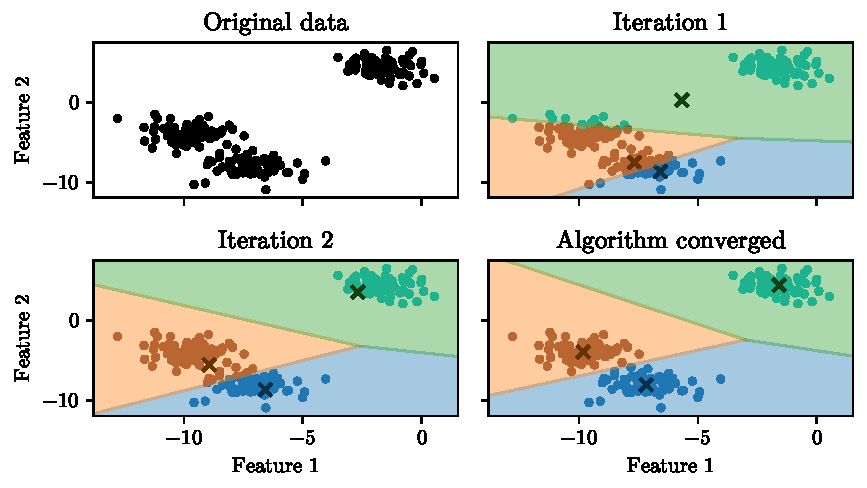
\includegraphics[width=\textwidth]{images/Kmeans/Kmeans_vornoi.pdf}
  \caption{K-means algorithm in the $2$-dimensional space}
  \label{fig:kmeans_vornoi}
\end{figure}

 The naive k-means algorithm consists of a series of iterations. First, the {\gls{glo:cent}}s $\gls{sym:cent}_i$ are initialized randomly, then the {\gls{glo:snap}}s are assigned to the nearest {\gls{glo:cent}}, and finally, the {\gls{glo:cent}}s are updated as the mean of the {\gls{glo:snap}}s assigned to them. These steps are repeated until the position of the {\gls{glo:cent}}s does not change anymore, or a defined maximum number of iterations is reached. This naive algorithm is summarized in the \autoref{alg:kmeans}.

\begin{algorithm}
  \caption{Training of the K-means model}
  \label{alg:kmeans}
  \begin{algorithmic}[1]
    \Function{K-means.train}{$\gls{sym:snapset}, k$}
    \LineComment{$\gls{sym:snapset}$ is the set of snapshots to be clustered}
    \LineComment{$k$ is the number of clusters to be obtained}
    \State $\gls{sym:cent}_i \gets \text{random initialization}, \forall i \in [1,k], \gls{sym:cent}_i \in \text{Domain of }\gls{sym:snapset}$
    \Repeat
    \LineComment{Every snapshot is assigned to the nearest centroid. Every centroid defines a cluster containing the assigned snapshots}
    \State $\gls{sym:cluster}_i \gets \left\{ \gls{sym:snap}_p : \norm{\gls{sym:snap}_p - \gls{sym:cent}_i}^2 \leq  \norm{\gls{sym:snap}_p - \gls{sym:cent}_j}^2  \forall j \in [1,k] \right\} \forall i \in [1,k] $
    \LineComment{The centroids are updated as the mean of their snapshots}
    \State $\gls{sym:cent}_i \gets \dfrac{1}{\abs{\gls{sym:cluster}_i}}\Sigma_{\gls{sym:snap}_j \in \gls{sym:cluster}_i} \gls{sym:snap}_j, \forall i \in [1,k]$, \Comment{$\abs{\gls{sym:cluster}_i}$ is the cluster size}
    \Until{All the centroids do not change anymore, or max iterations reached}
    \State $r_i \gets \max{\norm{\gls{sym:snap}_j-\gls{sym:cent}_i}, \, \forall \gls{sym:snap}_j \in \gls{sym:cluster}_i}, \, \forall i \in [1,k]$
    \State \Return $\mathcal{M}_{\text{\texttt{k-means}}}$  \Comment{The model contains the centroids $\gls{sym:cent}_i$, the radii ${r}_i$ of the clusters, and the labels of the snapshots}
    \EndFunction
  \end{algorithmic}
\end{algorithm}

As an example, we can consider $F=2$ features, and generate some test points shaped like three separated clusters. In the \autoref{fig:kmeans_vornoi} are shown the original data, the first two iterations of the algorithm, and the final result. The K-means algorithm had $n=200$ {\gls{glo:snap}}s, and $k=3$ clusters as input. The colors of the dots and the shaded areas represent the clusters and the decision boundaries. The {\gls{glo:cent}}s are represented as black crosses.
The decision boundaries are a Voronoi tessellation of the space, and they are defined as the set of points that are equidistant from the {\gls{glo:cent}}s of two different clusters. The algorithm itself does not compute the boundaries, but it is useful to plot them for visualization purposes.

\subsection{Variatons of the K-means algorithm}
\label{sec:kmeans_improvements}
\paragraph*{Kmeans}
Finding the optimal solution of the k-means problem (\autoref{eq:kmeans_problem}), as said, is NP-hard.
To address this problem, some other {\gls{glo:heuristic}}s algorithms have been proposed in the last two decades. Simple implementations have time complexity $\mathcal{O}(n^2)$ \cite{Kmeans_linear}.  This means that most algorithms do not scale well as the number $n$ of {\gls{glo:snap}} increases. With respect to the number of clusters, the problem has a linear complexity $\mathcal{O}(k)$.

It is worth noticing that an exact solution of the problem has been published \cite{Kmeans_vornoi_japan} with a time complexity $\mathcal{O}(n^{k\cdot F})$. This is still impractical for actual applications, as it is exponential with respect to both the number of clusters and the number of features $F$.

\paragraph*{Lloyd's algorithm}
The classic Lloyd algorithm \cite{Lloyd1982} has a complexity $\mathcal{O}(n\cdot k\cdot F )$.

\paragraph*{Various improvements to Lloyd's algorithm} Keeping the same basic idea, various modifications of the Lloyd algorithm have been proposed to improve the performances. For example, Kanugo \cite{kanungo2004local} proposed a local search algorithm that has a complexity $\mathcal{O}(n^3)$. Another result by Malay \cite{Kmeans_linear} has a linear complexity $\mathcal{O}(n)$. 

Another improvement has been developed by Elkan \cite{kmeans-accelerated}, by keeping track of the bounds from the instances ({\gls{glo:snap}}s) and the {\gls{glo:cent}}s. This algorithm becomes convenient when the number $k$ of clusters is large ($\geq 20$), and up to a dimensionality of $F=1000$ features.

A variant of the Lloyd algorithm regarding both the speed of execution and the memory consumption has been proposed by Sculley \cite{Sculley2010}. This solution achieves a reduction of the execution time by orders of magnitude and enables performing the classification even for datasets that don't fit in the memory of the machine. This is achieved by using a \emph{mini-batch} approach, where the {\gls{glo:cent}}s are updated after each batch of {\gls{glo:snap}}s.

Concerning the problem of converging to a local minimum, the most common approach is to run the algorithm multiple times with different initializations and then select the best result, this is avoided by Reddy \cite{Vornoi_Kmeans}, by using the Voronoi tessellation of the hyperspace using the datapoints to generate the initialization for the {\gls{glo:cent}} positions, this algorithm perform better in the sense that is less likely to get trapped in a local minimum.


\paragraph{K-means\texttt{++}} 
The last improved algorithm reported in this section has its own paragraph because it is the one used in this thesis. It was developed and named Kmeans\texttt{++} by Arthur and Vassilvitskii in 2007 \cite{Kmeanspp}. The difference from the Lloyd algorithm is only in the first initialization of the {\gls{glo:cent}}s $\gls{sym:cent}_i \forall i \in [1,n]$. In this case, instead of a random initialization for all the {\gls{glo:cent}}s, the first {\gls{glo:cent}} $\gls{sym:cent}_1$ is chosen randomly from the {\gls{glo:snap}}s, and then the other {\gls{glo:cent}}s are chosen from the remaining {\gls{glo:snap}}s with a probability that depends from the distance of the candidate {\gls{glo:snap}} to the closest already chosen {\gls{glo:cent}}. This approach is summarized in the \autoref{alg:kmeanspp}.

For the development of the framework of this thesis, the K-means\texttt{++} algorithm has been implemented in \texttt{Python}, using the \texttt{scikit-learn} library. The library function has been modified, adding a method that returns the radii of the clusters, this information is crucial for our scope, as it will be needed for evaluating if a new {\gls{glo:snap}} is a novelty, normal or fault, as it will be explained in the \autoref{sec:clust_metric} and \autoref{sec:clust_threshold}.

\begin{algorithm}
  \caption{K-means\texttt{++} algorithm}
  \label{alg:kmeanspp}
\begin{algorithmic}[1]
  \Function{K-means\texttt{++}.train}{$\gls{sym:snapset}, k$}
  \LineComment{$\gls{sym:snapset} = \{\gls{sym:snap}_1,\gls{sym:snap}_2, \dots , \gls{sym:snap}_n\}$ is the set of snapshots to be clustered}
  \LineComment{$k$ is the number of clusters to be obtained}
  \State $\gls{sym:cent}_1 \gets \text{random initialization}, \gls{sym:cent}_1 \in \gls{sym:snapset}$
  \For{$i \gets 2$ to $k$}
  \LineComment{$D(\gls{sym:snap})$ is the distance of the snapshot $\gls{sym:snap}$ from the closest centroid already chosen}
  \State $c_i \gets \gls{sym:snap}' \in \gls{sym:snapset} \text{ with probability } \dfrac{D(\gls{sym:snap}')^2}{\Sigma_{\gls{sym:snap}\in\gls{sym:snapset}}D(\gls{sym:snap})^2}$
  \EndFor
  \State perform the Lloyd algorithm using the calculated $\gls{sym:cent}_i, \forall i \in [1,k]$ as initialization, get the model.
  \State \Return $\mathcal{M}_{\text{\texttt{k-means}}}$  \Comment{The model contains the centroids $\gls{sym:cent}_i$, the radii ${r}_i$ of the clusters, and the labels of the snapshots}
  \EndFunction
\end{algorithmic}
\end{algorithm}

\subsection{Selecting the number of clusters}
It is important to notice that, even being an \emph{unsupervised} learning algorithm, the K-means algorithm needs to know the number of clusters $k$ in advance. There are some methods to decide what is the best number of clusters, but they usually need to perform more iterations of the algorithm with different values of $k$, and then compare the results. This task is automatable so, during the training phase, the user can decide the number of clusters to be used, or leave the selection to the algorithm itself.

To compare the results of the different iterations, it is possible to use some metrics on the data and the {\gls{glo:cent}}s. The most common metrics are the \emph{inertia} and the \emph{silhouette score}, described in the following paragraphs.

\paragraph*{Inertia}
The inertia metric measures the total (sum) distance of each point belonging to a cluster from the {\gls{glo:cent}} of the cluster itself, as shown in the \autoref{eq:inertia}. This is called inertia because, in the physical sense, it is the sum of the moment of inertia of each cluster if all the {\gls{glo:snap}}s were considered as point masses (with unitary mass). This analogy is useful to understand that the lower the inertia, the more compact the clusters are.

Let's span $k \in [1,9]$ and plot the inertia of the clusters for each value of $k$, on the previous dataset. The result is shown in the \autoref{fig:kmeans_inertia}. As expected, the inertia decreases as the number of clusters increases. This is not a desirable behavior, if the aim is selecting the number of clusters, the best guess is to select (by eye or with some automatism) the Pareto optimal point (\glsxtrshort{pof}) of the curve \cite{pareto}. 

\begin{equation}
  \label{eq:inertia}
  I = \sum_{i=1}^{k}\sum_{\gls{sym:snap}_j \in \gls{sym:cluster}_i} \norm{\gls{sym:snap}_j - \gls{sym:cent}_i}^2
\end{equation}

\begin{figure}
  \begin{subfigure}{\textwidth}
    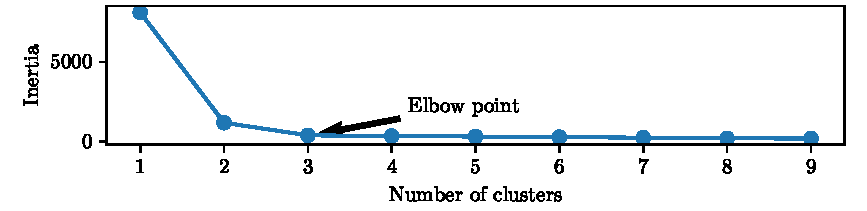
\includegraphics[width=\textwidth]{images/Kmeans/Kmeans_inertia.pdf}
    \caption{Inertia of the clusters for different values of $k$}
    \label{fig:kmeans_inertia}
  \end{subfigure}
  \begin{subfigure}{\textwidth}
    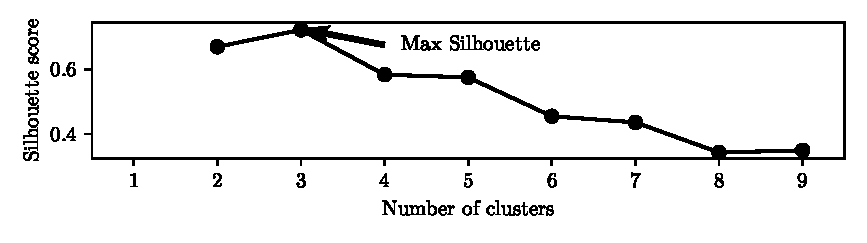
\includegraphics[width=\textwidth]{images/Kmeans/Kmeans_silhouette.pdf}
    \caption{Silhouette score of the clusters for different values of $k$}
    \label{fig:kmeans_silhouette}
  \end{subfigure}
  \label{fig:kmeans_metrics}
  \caption{Metrics for selecting the number of clusters}
\end{figure}

\paragraph*{Silhouette score}
A better metric that can be used to select the number of clusters is the silhouette score.
The silhouette score is defined for each {\gls{glo:snap}} as in \autoref{eq:silhouette}, where $a$ is the mean distance of the {\gls{glo:snap}} from the other {\gls{glo:snap}}s in the same cluster, and $b$ is the mean distance of the {\gls{glo:snap}} from the {\gls{glo:snap}}s in the nearest cluster. The resulting silhouette $S_i$ of a {\gls{glo:snap}} $\gls{sym:snap}_i$ is a scalar: $S_i \in [-1,1]$.
The three relevant cases are:
\begin{itemize}
  \item a value close to $1$ means that the {\gls{glo:snap}} is far inside its own cluster and far from {\gls{glo:snap}}s of other clusters;
  \item a value close to $0$ means that the {\gls{glo:snap}} is on the boundary between two clusters;
  \item a value close to $-1$ means that the {\gls{glo:snap}} is far from its own cluster and close to another cluster, so it may have been misassigned.
\end{itemize}

\begin{equation}
  \label{eq:silhouette}
  S_i = \frac{b_i - a_i}{\max{(a_i,b_i)}}
\end{equation}

At this point, the global silhouette score $S_g$ can be computed as the mean of the silhouette scores of all the {\gls{glo:snap}}s (\autoref{eq:silhouette_global}). The global silhouette score, for the same example dataset, is shown as a function of the number of clusters $k$ in the \autoref{fig:kmeans_silhouette}. Note that this time $k \in [2,9]$, because the silhouette score is not defined for a single cluster.

In this case, the best value for $k$ is $k=3$, because it is the value that maximizes the silhouette score. This approach is simpler and easier to automate than the inertia one. 

\begin{equation}
  \label{eq:silhouette_global}
  S_g = \frac{1}{n}\sum_{i=1}^{n} S_i
\end{equation}

\subsection{Assignation of the new instance to a cluster}
The procedure for assigning the new {\gls{glo:snap}} $\gls{sym:snap}_n$ to a cluster is quite simple, it is sufficient to compute the distance between $\gls{sym:snap}_n$ and the {\gls{glo:cent}}s $\gls{sym:cent}_m$, $\forall m \in  [1, \dots , k]$. The distance is defined as the $l^2$-norm in the feature space, it can be computed using the \autoref{eq:clust_dist}, and assign $\gls{sym:snap}_n$ to the cluster with the minimum distance.

\begin{equation}
  \label{eq:clust_dist}
  \gls{sym:dist}_{n,m} = ||\gls{sym:snap}_{n,f} - \gls{sym:cent}_{m,f}||_2 = \sqrt{\sum_{f=1}^{F} (\gls{sym:snap}_{n,f} - \gls{sym:cent}_{m,f})^2}
\end{equation}

\subsection{Evaluation of a new instance}

At this point, with a model trained on the data, a generic $n$th new {\gls{glo:snap}} instance $\gls{sym:snap}_n$ can be evaluated using the K-means algorithm.
From a geometric point of view, the {\gls{glo:snap}} $\gls{sym:snap}_n$ is a point in the ${F}$-dimensional space, where ${F}$ is the number of features used to train the model.

For demonstration purposes, in this section, since it is still feasible to show 3D plots, it is considered an example with ${F}=3$ features.

\begin{figure}[htbp]
  \centering
  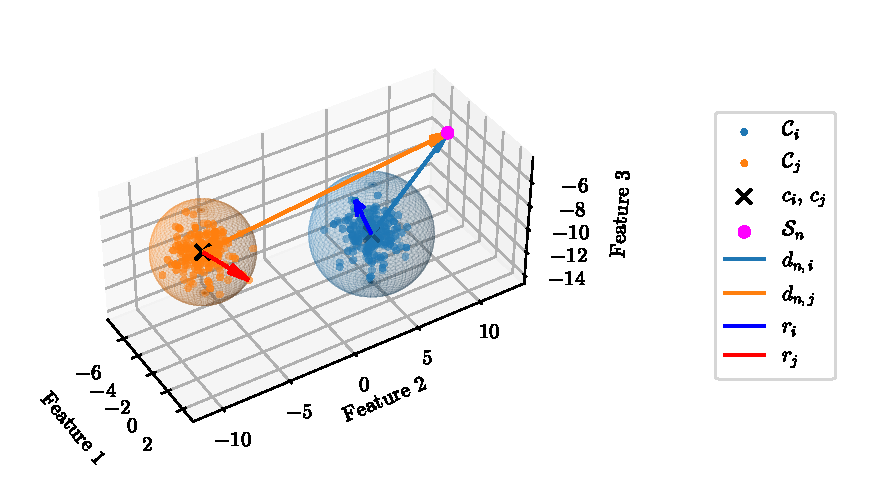
\includegraphics[width=\textwidth]{images/Kmeans/Spheres_2.pdf}
  \caption{Cluster model in the $3$-dimensional space, with new snapshot $\gls{sym:snap}_n$}
  \label{fig:clust_spheres}
\end{figure}

In the \autoref{fig:clust_spheres}, the training data are represented in the $3$-dimensional space, where the axis are the features used to train the model. The K-means model has been ideally trained with an arbitrary number $k$ of clusters but, for display purposes, only two clusters  ($\gls{sym:cluster}_i$ and $\gls{sym:cluster}_j$) are plotted.
\paragraph*{}
The entities shown in the \autoref{fig:clust_spheres} are:
\begin{itemize}
  \item $\gls{sym:cent}_{i(j)}$ is the centroid of the $i$th ($j$th) cluster;
  \item $\gls{sym:radius}_{i(j)}$ is the radius of the $i$th ($j$th) cluster, it is defined as the distance between the centroid $\gls{sym:cent}_{i(j)}$ and the farthest point belonging to the cluster itself;
  \item $\gls{sym:cluster}_{i(j)}$ is the set of training snapshots belonging to the $i$th ($j$th) cluster, it has a centroid $\gls{sym:cent}_{i(j)}$ and a radius $\gls{sym:radius}_{i(j)}$;
  \item $\gls{sym:snap}_n$ is the new snapshot to be evaluated;
  \item $\gls{sym:dist}_{n,i}$ is the vector between $\gls{sym:snap}_n$ and $\gls{sym:cent}_i$;
  \item $\gls{sym:dist}_{n,j}$ is the vector between $\gls{sym:snap}_n$ and $\gls{sym:cent}_j$;
  \item the semi-transparent spheres represent the cluster sizes, the radius of the spheres is the radius of the cluster itself, and the center is the centroid of the cluster;
\end{itemize}



\subsection{Metric for the new instance evaluation}
\label{sec:clust_metric}
Once the new {\gls{glo:snap}} $\gls{sym:snap}_n$ has been assigned to the right cluster $\gls{sym:cluster}_i$ using \autoref{eq:clust_dist}, some kind of measure (\gls{aka} metric) linked to how novel this {\gls{glo:snap}} is needs to be computed. In this document, this measure, referred to the $n$-th cluster, will be called $e_n$, in order to remind some sort of error, even if it is not an error in the strict sense. One simple approach could be to compute the difference between the distance of $\gls{sym:snap}_n$ from the {\gls{glo:cent}} $\gls{sym:cent}_i$ and the radius $\gls{sym:radius}_i$ of the cluster itself. With this approach, the measure defined in the \autoref{eq:clust_eval} is relative to the current {\gls{glo:snap}}, so it is possible to use that as a novelty measure.

\begin{equation}
  \label{eq:clust_eval}
  e_{n} = ||\gls{sym:dist}_{n,i}||_2 - ||\gls{sym:radius}_{i}||_2, \text{ where $i$ is the of the assigned cluster}
\end{equation}

Few consideration about the resoult of the \autoref{eq:clust_eval}:
\begin{itemize}
  \item if $e_{n} > 0$, the new {\gls{glo:snap}} $\gls{sym:snap}_n$ is outside the sphere of radius $\gls{sym:radius}_i$ centered in $\gls{sym:cent}_i$, so it is probably a novel {\gls{glo:snap}};
  \item if $e_{n} < 0$, the new {\gls{glo:snap}} $\gls{sym:snap}_n$ is inside the sphere of radius $\gls{sym:radius}_i$, so it is probably a normal {\gls{glo:snap}}. In this case, it is worth noticing that this assumption is reasonable only if the shape of the point cloud resembles a sphere, otherwise, the radius $\gls{sym:radius}_i$ is not a good measure of the cluster size, and use it for novelty detection would not be reasonable. \textbf{This emphasizes the importance of the standardization procedure applied to the features before the training phase};
\end{itemize}



Using this metric it is possible to define as \emph{novelty} all the {\gls{glo:snap}}s with $e_{n} > 0$ and as \emph{normal} all the {\gls{glo:snap}}s with $e_{n} < 0$. This approach is not very robust because s {\gls{glo:snap}} that is even slightly outside the sphere of radius $\gls{sym:radius}_i$ will be considered as novelty, but since the sphere is tuned the training \emph{measured} data, that have an aleatory component, this approach will probably detect some novelty even in normal {\gls{glo:snap}}s.

\subsection{Introducing a threshold for the metric evaluation}
\label{sec:clust_threshold}
In order to improve the robustness of the novelty detection algorithm, it is possible to define a threshold ${t}_i$ for each cluster $\gls{sym:cluster}_i$ and use it to detect if a {\gls{glo:snap}} is a novelty or not. Once the threshold ${t}_i$ is defined, the detection of the novelty can be triggered by the condition $e_{n} > {t}_i$.

\paragraph*{}
At this point, the problem is that the user would have to define a threshold for each cluster, and this is not a trivial task. This is because it is likely that the clusters have different sizes, and so one threshold for all the clusters would be more conservative for the smaller clusters and less conservative for the bigger ones. Moreover, most of the times, the clusters' shape and size will not have a physical meaning, and the act of manually defining a threshold for each cluster would go against our goal of designing a fully unsupervised framework.

\paragraph*{}
To address this problem, it is possible to change the definition of the metric itself, so that is not dependent on the cluster size. This can be done by normalizing the already defined metric $e_{n}$ with the radius $\gls{sym:radius}_i$ of the cluster itself, as shown in the \autoref{eq:clust_eval_norm}. In this way, $t_i$ can be defined as a percentage of the cluster size, so that the user can define a single threshold for all the clusters, and selecting the number to assign to $t_i$ has a more intuitive meaning. From now on if not otherwise specified, the metric $e_{n}$ will be this normalized version.
Obviously, the metric can be easily displayed as a percentage: $e_{n,\%} = e_n \cdot 100$.
This value can be evaluated in real-time and plotted in a graph so that the user can see the novelty metric behavior over time.

\begin{equation}
  \label{eq:clust_eval_norm}
  e_{n} = \frac{\norm{\vect d_{n,i}}-\norm{\vect r_{n,i}}}{\norm{\vect r_{n,i}}} = \frac{\norm{\gls{sym:dist}_{n,i}}}{\norm{\gls{sym:radius}_{i}}} - 1, \text{ where $i$ is the of the assigned cluster}
\end{equation}

After applying this scaling, the metric now follows this rule of thumb:
\begin{itemize}
  \item $e_n \in [-1,0] \implies \gls{sym:snap}_n$ is a normal {\gls{glo:snap}};
  \item $e_n \in (0,+\infty) \implies \gls{sym:snap}_n$ is a novelty;
\end{itemize}

\subsection{Trasformation of the metric for the fault detection}
\label{sec:clust_fault}
In the previous \autoref{sec:clust_threshold} a metric has been proposed to detect how novel a {\gls{glo:snap}} is.

Let's assume now to have trained the model on a dataset of {\gls{glo:snap}}s collected in a period in which the system was having a known malfunction. In this case, the metric applied to any future {\gls{glo:snap}} will carry the information of \quoted{how faulty} the system is, or better \quoted{how similarly the system is behaving \gls{wrt} a known malfunction}.

Since the metric already defined is the normalized distance of the current \gls{glo:snap} from the {\gls{glo:cent}} of the cluster, if the clustered data are indicative of a malfunction, the metric $e_n$ will be in the range $[-1,0]$ when the system has a known malfunction present in the training data and $e_n$ will be in the range $(0,+\infty)$ when the system is not behaving as a known malfunction.

To maintain the same behavior of the metric as in \autoref{sec:clust_threshold}, a trasformation that maps the range $[-1,0]$ into $(0,+\infty)$, and the range $(0,+\infty)$ into $[-1,0]$ is needed. This can be done by applying a logarithmic transformation to the metric, as shown in the \autoref{eq:clust_eval_log}. This transformation is applied only if the model is working in fault detection mode, otherwise, the metric has to remain the same as in \autoref{eq:clust_eval_norm}.

\begin{equation}
  \label{eq:clust_eval_log}
  e'_{n} = -\ln(e_n+1) = -\ln{\left(\frac{\norm{\gls{sym:dist}_{n,i}}}{\norm{\gls{sym:radius}_{i}}}\right)}, \text{ where $i$ is the the assigned cluster}
\end{equation}

In practice, to avoid numerical representation problems, it is mandatory to avoid mapping $-1$ (when the new snapshot happens to be perfectly in the center of a cluster) into $+\infty$. To do that, a constant slightly smaller than $1$ is multiplied to the metric before applying the logarithmic transformation, so that the function will have the vertical asymptote slightly before $-1$, and all the inputs $\in [-1,0]$ will be mapped into real values. The plot of the settled function is shown in the \autoref{fig:kmeans_fault}.

\begin{figure}[htbp]
  \centering
  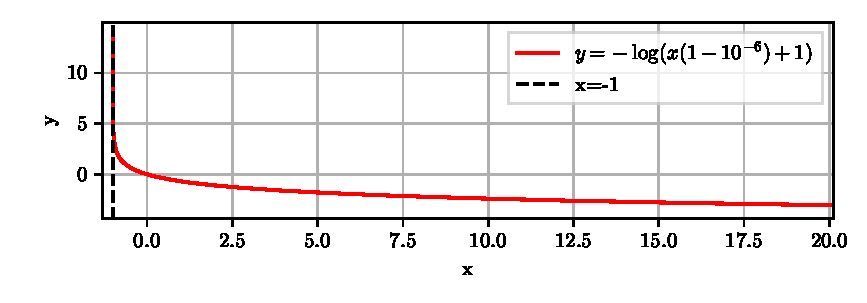
\includegraphics[width=\textwidth]{images/kmeans/metric_trasform.pdf}
  \caption{Logarithmic Transformation applied to the metric in case the model is working in fault detection mode}
  \label{fig:kmeans_fault}
\end{figure}


\subsection{Evaluation procedure}
The evaluation procedure developed to address the novelty/fault detection scope of this thesis can be summarized in the \autoref{alg:eval_new_snapshot}.

\begin{algorithm}
  \caption{Evaluation of a new snapshot with a K-means model}
  \label{alg:eval_new_snapshot}
  \begin{algorithmic}[1]
    \Procedure{eval}{$\mathcal{M}_{\text{\texttt{k-means}}},\gls{sym:snap}, t$}
    \LineComment{$\mathcal{M}_{\text{\texttt{k-means}}}$ is the trained K-means model}
    \LineComment{the model contain the centroids $\gls{sym:cent}_i$ and the radii $\gls{sym:radius}_i$ of the clusters}
    \LineComment{$\gls{sym:snap}$ is the new snapshot to be evaluated}
    \LineComment{$t$ is the threshold for the novelty detection}
    \State $k \gets \text{number of clusters in $\mathcal{M}_{\text{\texttt{k-means}}}$}$
    \State min $\gets \infty$ \Comment {initialize the minimum distance}
    \For{$i \gets 1$ to $k$}
    \State $\gls{sym:dist}_{i} \gets \gls{sym:snap} - \gls{sym:cent}_{i}$
    \If {$\norm{\gls{sym:dist}_{i}} < \text{min}$}
    \State min $\gets \norm{\gls{sym:dist}_{i}}$
    \State $i_{\text{min}} \gets i$
    \EndIf
    \EndFor
    \State$e \gets \dfrac{\norm{\gls{sym:dist}_{i_{\text{min}}}}}{\norm{\gls{sym:radius}_{i_{\text{min}}}}} - 1$ \Comment {compute the novelty metric}
    \If {fault detection mode}
    \State $e \gets -\ln(e\cdot(1-10^-6)+1)$ \Comment {apply the logarithmic trasformation}
    \EndIf
    \If {$e > t$}
    \State \Return novelty flag, $e$  \Comment {the snapshot is novelty}
    \Else
    \State \Return normal flag, $e$ \Comment {the snapshot is normal}
    \EndIf
    \EndProcedure
    %\end{small}
  \end{algorithmic}
\end{algorithm}


\subsection{Comment about selecting the wrong value of $k$}
\label{sec:wrong_k}
A brief comment about what has been done in the experimental phase, in the cases where the number of clusters $k$ was difficult to define based on the silhouette plots. This happened when the maximum value of $k$ was shared between more than one value of $k$ (multiple peaks with similar values or a flat shape of the peak).

In this case, the best choice is to select the maximum value of $k$ that is still compliant with the silhouette criterion. This is because the in scope of this thesis the final goal is to detect novelty. 

For display purposes, let's consider an example in the plane ($F$ = 2), with a dataset that clearly has three distinct clusters. Looking at \autoref{fig:kmeans_wrongk} it is clear why it is better to select $k$ larger than the actual number of clusters, rather than selecting it too small. This is because, if $k$ is larger than the actual number of clusters, the algorithm will still be able to detect the novelty, but if $k$ is too small, somewhere the algorithm will be forced to join two clusters together, and a new {\gls{glo:snap}} that happens to be in the middle of the two clusters will not be detected as novelty. 

In the case of the \autoref{fig:kmeans_wrongk}, the best actual number of clusters was $k=3$, so selecting $k=2$ the algorithm would have joined the two clusters on the right, and the new {\gls{glo:snap}} would not have been detected as novelty. On the other hand, by selecting $k=4$, the algorithm would have correctly detected the novelty, even if one cluster had been split in two.

\begin{figure}
  \centering
  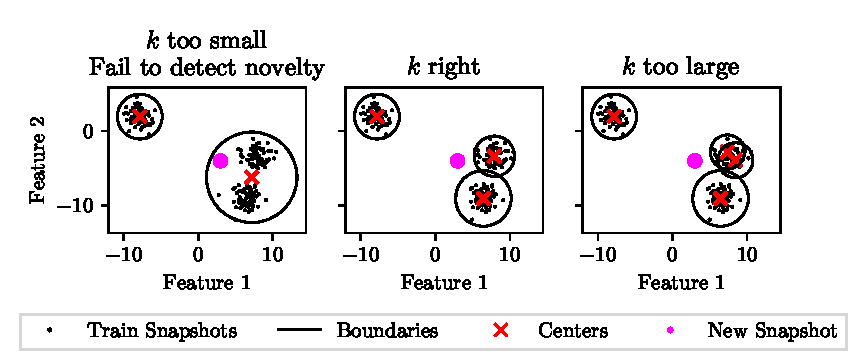
\includegraphics[width=\textwidth]{images/Kmeans/Kmeans_wrongk.pdf}
  \caption{Novelty detection of a new $\gls{sym:snap}_j$ with different values of $k$}
  \label{fig:kmeans_wrongk}
\end{figure}


\subsection{Limits of the k-means algorithm}
\label{sec:kmeans_limits}
This algorithm has many advantages: it's simple, popular (easy to find in libraries), it's fast, produces a model that does not need to store the original data in order to perform the classification of a new instance and is well scalable. But it has also some limits, the most important are \citepage{hands-on-geron2022}{273}:
\begin{itemize}
  \item it performs poorly if the clusters are not spherical;
  \item it performs poorly if the clusters have very different sizes;
  \item it performs poorly if the clusters have different densities.
\end{itemize}

For this reason it is very important to perform a good preconditioning of the data. In this thesis, the data are \gls{glo:std} before the training phase, this makes the clusters more spherical and with similar sizes. 




\section{DBSCAN}
\label{sec:dbscan}

\begin{figure}[htbp]
    \centering
    \begin{subfigure}{\textwidth}
    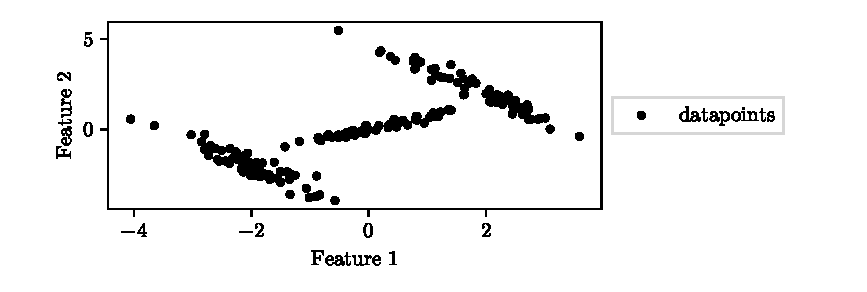
\includegraphics[width=\textwidth]{images/DBSCAN/Figure_1.pdf}
    \caption{training data}
    \end{subfigure}
    \begin{subfigure}{\textwidth}
    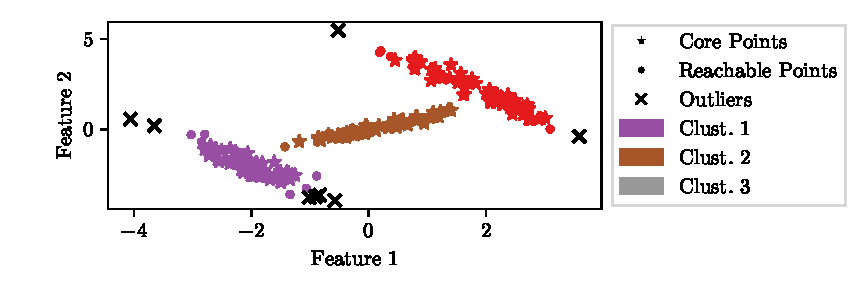
\includegraphics[width=\textwidth]{images/DBSCAN/Figure_2.pdf}
    \caption{training result}
    \end{subfigure}
    \caption{DBSCAN clustering}
    \label{fig:dbscan}
\end{figure}
\section{Gaussian Mixture Model}
\label{sec:gaussian}

\begin{figure}
    \centering
    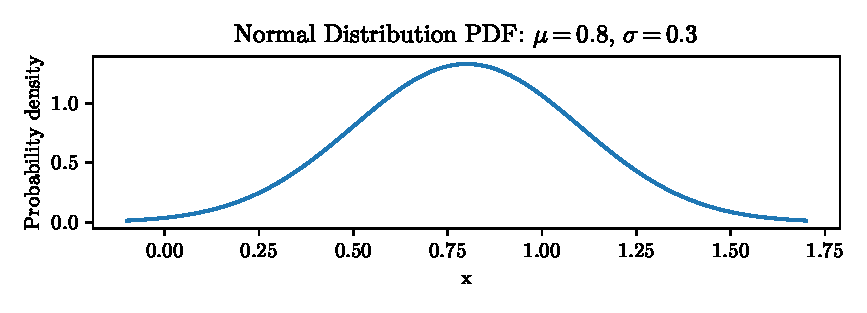
\includegraphics{images/Gaussian/Figure_3.pdf}
    \caption{Gaussian distribution probability density function}
    \label{fig:gauss_pdf}
\end{figure}

The \autoref{fig:gauss_pdf} illustrates a Gaussian distribution probability density function (\gls{pdf}), also known as normal distribution. The peak represents the mean $\mu$, while the spread is determined by the standard deviation $\sigma$. The equation of the \gls{pdf} is the following:

$$
f(x) = \frac{1}{\sigma \sqrt{2\pi} } e^{-\frac{1}{2}\left(\frac{x-\mu}{\sigma}\right)^2}
$$

\paragraph*{}
A Gaussian Mixture Model is a probabilistic model that assumes that the data are generated from a mixture of several Gaussian distributions. Depending on the parameters of a Gaussian distribution (mean and variance) on each axis (Features), the data generated from it in the $\gls{sym:feats}$-dimensional space will have a shape that resembles an ellipsoid with a centre and an orientation.


\subsection{Training}
\label{sec:gauss_train}
As anticipated, the assumption is that every \gls{glo:clust} has a normal \gls{pdf} on each axis. So, for each \gls{glo:feature}, the total \gls{pdf} is a superposition of $k$ normal \gls{pdf}. 
The algorithm used to train the model is the Expectation Maximization (\gls{em}) algorithm. This is a generalization of the k-means algorithm that allows to find the centroids (means), the covariance matrices of the \gls{glo:clust}s, and their weights. Unlike the k-means, the \gls{em} is a soft \gls{glo:clust}ing algorithm, meaning that each point is assigned to each \gls{glo:clust} with a probability, instead of being assigned to a single \gls{glo:clust}.
The \gls{em} algorithm is an iterative algorithm that aims to find the parameters that maximize the \gls{glo:likelihood}.

\subsection{Selecting the number of \gls{glo:clust}s}
\begin{figure}[htbp]
    \centering
    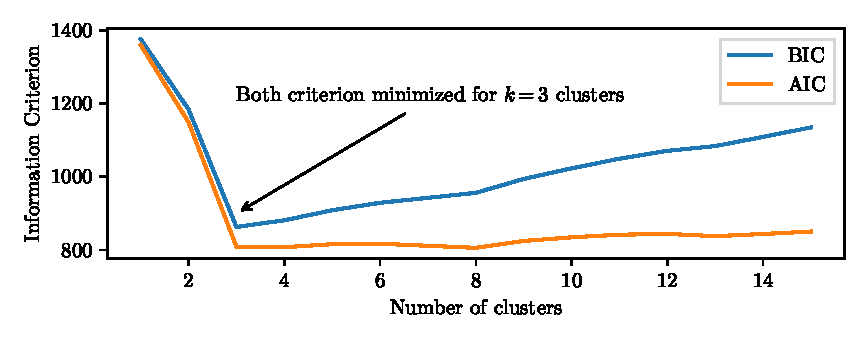
\includegraphics{images/Gaussian/Figure_1.pdf}
    \caption{Criteria for selecting the number of \gls{glo:clust}s}
    \label{fig:gauss_criterion}
\end{figure}
In \autoref{sec:gauss_train} we have seen that the \gls{em} algorithm needs to know in advance the number of \gls{glo:clust}s $k$ to train the model. To select the best $k$ we could use the same criteria used for the k-means, that is the elbow method or the silhouette score. But, since the \gls{em} is most suitable for ellipsoids-shaped \gls{glo:clust}s of very different sizes, it is better to avoid those metrics that work best with spherical \gls{glo:clust}s. Instead, we can use the \gls{aic} or the \gls{bic} criteria, which are functions of the size $m$ of the training dataset, the number $p$ of parameters, and the max value of \gls{glo:likelihood} $\hat{\mathcal{L}}$.

\begin{equation}
    \begin{matrix}
        \gls{aic} &=& 2p - 2 \ln(\hat{\mathcal{L}}) \\
        \gls{bic} &=& p \ln(m) - 2 \ln(\hat{\mathcal{L}})
    \end{matrix}
    \label{eq:aic_bic}
\end{equation}

Both the criteria in \autoref{eq:aic_bic} penalize the models with a large number of parameters, they usually select the same model, but if they select different models, the \gls{aic} tends to select the most accurate model.

Considering, as an example, the same dataset used in \autoref{fig:dbscandata}, and running the \gls{em} algorithm with different values of $k$, we obtain the results shown in \autoref{fig:gauss_criterion}. As expected the \gls{aic} and the \gls{bic} criteria select the same model, that is the one with $k=3$.

\subsubsection{Totally automated approach}
\label{sec:gauss_unsupervised}
Another advantage of the \gls{gmm} is that it can be used in a totally automated way. This can be done using the variation called Bayesian Gaussian Mixture Model \gls{bgmm}. This variation is able to assign $0$ as 
weight to some \gls{glo:clust}s, meaning that those \gls{glo:clust}s are not used to generate the \gls{pdf} of the samples. In this case, we can set the number of \gls{glo:clust}s as high as the size of the training dataset, and the \gls{bgmm} will select the best number of \gls{glo:clust}s to use to generate the \gls{pdf} of the samples. 

\subsection{Evaluation of a new instance}
\label{sec:gauss_eval}
\begin{figure}
    \centering
    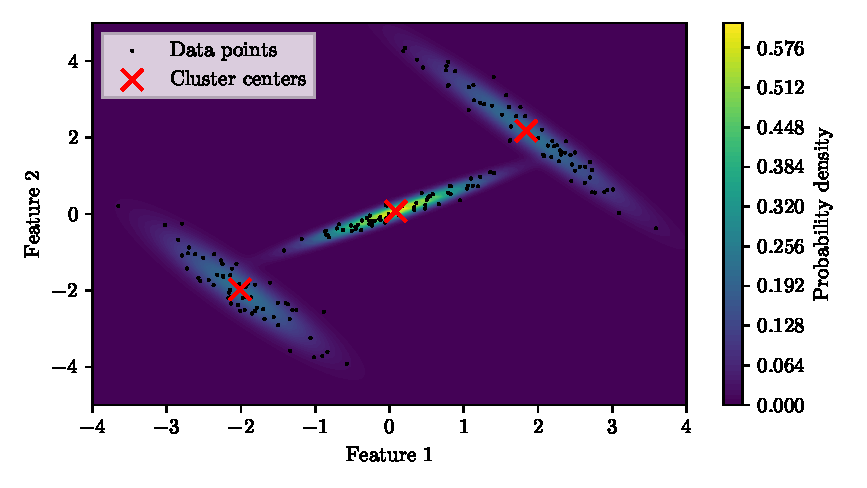
\includegraphics{images/Gaussian/Figure_2.pdf}
    \caption{Trained Gaussian Mixture Model}
    \label{fig:gauss_example}
\end{figure}
Once the model is well-trained, we can use it to evaluate a new instance. The \autoref{fig:gauss_example} shows the result of the training of the \gls{gmm} on the example dataset. The ellipsoids represent the \gls{glo:clust}s, the size of the ellipsoids is proportional to the weight of the \gls{glo:clust}, while the orientation and the size of the ellipsoids are determined by the covariance matrix of the \gls{glo:clust}. 

The \texttt{pyhton} implementation of the \gls{gmm} used in this project is the one provided by the \texttt{sklearn} library. It has an attribute called \texttt{score\_samples} that returns the log value of the \gls{pdf} of the samples.
The bigger the value, the more likely it is to be inside a \gls{glo:clust}. 
To maintain the same philosophy of the other algorithms, we can take the negative value of \texttt{score\_samples} as a metric to evaluate the novelty of a new instance. 

\subsubsection{Selecting the threshold}
As said for K-means, and \gls{dbscan}, a threshold will be needed to decide if the new instance is novel or not. If, as supposed for now, the scenario is that the training dataset is composed only of normal instances, then the threshold can be selected by looking at the distribution of the novelty metric on the training dataset and selecting a value slightly higher than the maximum value for the training dataset.

If the scenario is that the training dataset is composed of both normal and anomalous instances sampled at constant intervals, and the ratio between normal and anomalous instances is known, then \gls{gmm} enables us to select the threshold in a more sophisticated way.

Suppose for example that $1\%$ of the training dataset is anomalous, since the model gives us the \gls{pdf} of the samples, we can compute the threshold as the $1\%$ percentile of the \gls{pdf} of the training dataset. This will ensure that the $1\%$ of the training instances will be classified as anomalous. If the model is correct, also future evaluations will have the same ratio of anomalous instances.

\subsection{Limitations of the algorithm}
The main limitation of the \gls{gmm} is that it is not able to identify \gls{glo:clust}s with arbitrary shapes.

If the data are not shaped like some ellipsoids, the model can approximate the data anyway, splitting the \gls{glo:clust}s into smaller ellipsoids. For our purposes of novelty detection, this is not a limitation.

The complexity of the algorithm is $\mathcal{O}(kmF^2+kF^3)$, where $k$ is the number of \gls{glo:clust}s, $m$ is the number of samples, and $F$ is the number of \gls{glo:feature}s \citepage{hands-on-geron2022}{281}. This means that the algorithm is not scalable to a large number of \gls{glo:feature}s, but it is scalable to a large number of samples.
For our purposes, it's more important to have an algorithm that is fast to evaluate a new instance, than an algorithm that is fast to train.
\section{Isolation Forest}
\label{sec:IsolationForest}

Similarli to the Random Forest, that is used for classification, the Isolation Forest is an ensemble method that is used for anomaly detection. The idea is to train the decision trees to isolate the data from each other, rather than profiling the normal data, and then provide a score that represents how isolated the data is. The more isolated the data is, the more likely it is to be an anomaly. This algorithm was introduced in 2008 by \cite{iforest}, the paper also provides a way of computing the anomaly score.

This algorithm has the advantage of being very fast to train and requiring very little memory. For hour purposes, as previously said, it is more important to have an algorithm that is fast to evaluate a new instance, than an algorithm that is fast to train.

\subsection{Training}
The algorithm is available in \texttt{sklearn} library, and it is very easy to use. This is a trurly unsupervised algorithm, the function only takes the dataset as input, and manages to automatically select all the rest of the parameters. As an example, i used the same dataset used in the previous sections for the \gls{dbscan} and {\gls{gmm}} algorithms. The result is shown in \autoref{fig:IsolationForest}.

\begin{figure}
    \centering
    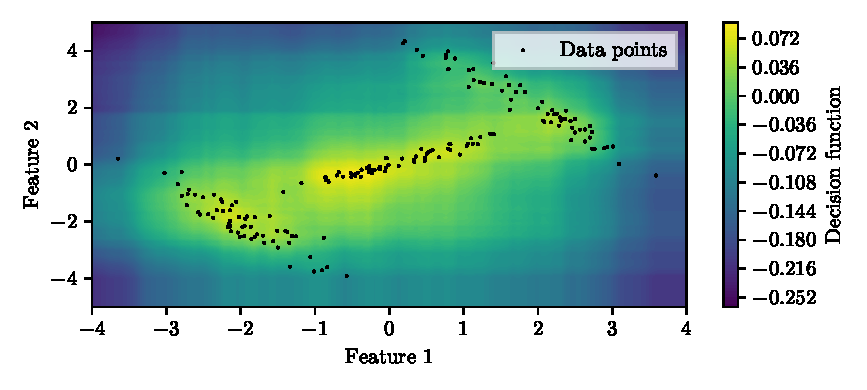
\includegraphics{images/IForest/Figure_1.pdf}
    \caption{Isolation Forest decision function.}
    \label{fig:IsolationForest}
\end{figure}

\subsection{Evaluation of a new instance}
\label{sec:iforest_eval}
The implementation in \texttt{sklearn} provides a function called \texttt{decision\_function}, plotted as an heatmap in \autoref{fig:IsolationForest}. the higher the value, the more likely it is to be a normal instance.
To mantain coherence with the work done up to now, we can take the negative value of \texttt{decision\_function} as a metric to evaluate the novelty of a new instance.

\subsection{Selecting the threshold}
\label{sec:iforest_threshold}
With this algorithm is it difficult to geometrically inerpret the decision function, so it is not possible to select the threshold a-priori. The approach could be to look at the values of the decision function on the training dataset, and select a value slightly higher than the maximum value for the training dataset.

\subsection{Limitations of Isolation Forest}
The main limitation is that since the algorithm is based on decision trees, the decision thresholds are defined on the features axis, so the decision boundaries are highly dependent on the clusters alignment with the axis. lokking back to \autoref{fig:IsolationForest}, we can see that the decision function has roughly the same value in the lower right corner as in the lower left corner, even if the lower right corner is clearly more isolated than the lower left corner. This is because the decision boundaries are aligned with the axis, and the lower right corner is more isolated only on the diagonal direction.

The complexity of the training phase is $\mathcal{O}(t\psi\log\psi)$ where $t$ is the number of trees used, and $\psi$ is the size of the subsampling size. The complexity of the evaluation is instead $\mathcal{O}(t\log\psi)$ \cite{iforest}.
\section{Local Outlier Factor}
\label{sec:LocalOutlierFactor}


The Local Outlier Factor (\gls{lof}) algorithm is effective in identifying outliers by assessing the density of instances surrounding a particular data point in comparison to the density around its neighbouring points. Typically, an anomaly is considered more isolated than its k nearest neighbours \citepage{hands-on-geron2022}{293}. 

Formally, the authors that designed this algorithm define the \gls{lof} of an instance $\gls{sym:snap}$ as the average of the ratio of the local reachability density of $\gls{sym:snap}$ and the local reachability density of its $MinPts$ k-nearest neighbours \cite{breunig2000lof}. This is a measure of how isolated the instance is with respect to the surrounding neighbourhood. 

Using this approach, this algorithm is able to identify outliers in a dataset with arbitrary shapes. Moreover, it can identify outliers in a dataset with different densities, as a point very near to a very dense cluster can be declared as an outlier, while a point even more distant from a less dense cluster could be declared as normal.

\subsection{Training}
\label{sec:lof_train}
\begin{figure}
    \centering
    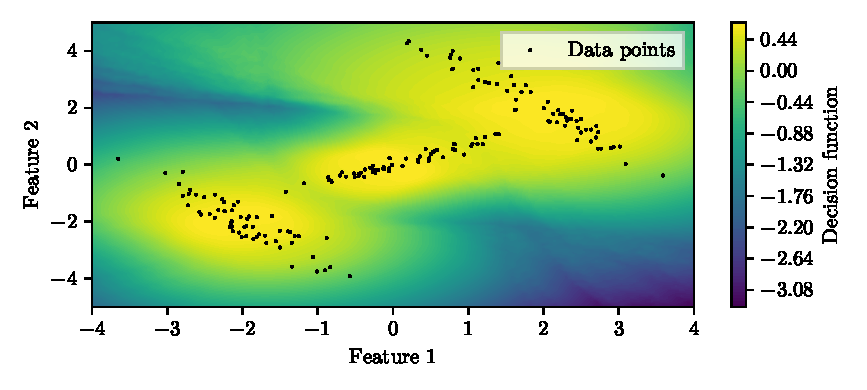
\includegraphics{images/LOF/Figure_1.pdf}
    \caption{Local Outlier Factor decision function.}
    \label{fig:LocalOutlierFactor}
\end{figure}
This algorithm is implemented in \texttt{sklearn} library and requires the number $MinPts$ of k-nearest neighbours to be specified. According to the authors, the value of \gls{lof} of a particular snapshot is neither increasing nor decreasing with the value of $MinPts$. They also suggest an \gls{glo:heuristic} to select the value of $MinPts$ that is hardly automatable. 
For this reason, it's difficult to use this algorithm in a real-time scenario in an unsupervised way.

Anyway, as an example, using the same dataset used in \autoref{fig:dbscandata}, and running the \gls{lof} algorithm with the default value of $MinPts=20$, we obtain the results shown in \autoref{fig:LocalOutlierFactor}.

\subsection{Evaluation of a new instance}
\label{sec:lof_eval}
The \texttt{sklearn} implementation of the \gls{lof} algorithm has a method that returns the \gls{lof} of a new instance. Since the bigger the value is, the more likely it is that the new snapshot is an outlier, we can take directly this value as a metric to evaluate the novelty of a new instance.

To select a threshold value, it holds what has been said in \autoref{sec:iforest_threshold} about \gls{iforest}.


\subsection{Limitations of Local Outlier Factor}
\label{sec:lof_limitations}
The main limitations are the difficulty of defining a threshold value to declare some instances as outliers and using this algorithm in a completely unsupervised way.



\section{One-Class Support Vector Machine}
\label{sec:OneClassSupportVectorMachine}

This algorithm is based on the kernelized \gls{svm} algorithm. While the standard application is to find the hyperplane that separates two classes, in this case, the aim is to separate the instances from the origin. If a new instance is too close to the origin (of an augmented hyperspace), then it is considered an outlier. It was introduced in 2001 by M\"{u}ller \cite{mullerOneClassSVM}.

\subsection{Training}
As an example, we refer to the same dataset used in the previous sections for the \gls{dbscan} and {\gls{gmm}} algorithms. The training of the version implemented in \texttt{sklearn} requires specifying the kernel to use, and the parameter $\nu$ that is the upper bound on the fraction of outlier. Training the algorithm on the dataset, with Gaussian kernel and $\nu=0.002$, we obtain the result shown in \autoref{fig:OneClassSupportVectorMachine}. 

\begin{figure}
    \centering
    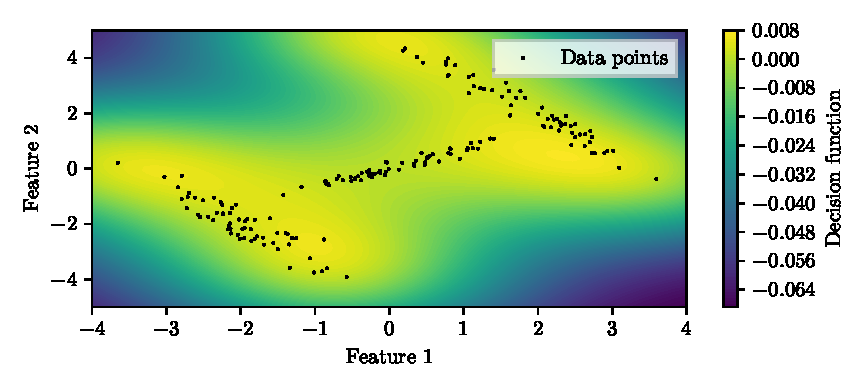
\includegraphics{images/nuSVM/Figure_1.pdf}
    \caption{One-Class Support Vector Machine decision function.}
    \label{fig:OneClassSupportVectorMachine}
\end{figure}

\subsection{Evaluation of a new instance}
\label{sec:svm_eval}
The decision function is the relative distance from the separation hyperplane, if it is positive, then the instance is considered normal, if it is negative, then the instance is considered an outlier. 

This allows us to take directly the negative of this value as a metric to evaluate the novelty of a new instance (to maintain coherence with previous sections). 

Furthermore, similarly to the \gls{gmm} case (\autoref{sec:gaussian}), if the training dataset contains only normal instances, we have to guess a positive value for the threshold by looking at the value of the metric on the training dataset, but if we have a dataset with a known fraction of outliers, we can use the fact that $\nu$ is the upper bound on the fraction of outliers to select $\nu$ correctly in the training phase, and then use a threshold of zero for the decision function. This should make at most a $\nu$ fraction of future evaluation to be considered outliers.

\subsection{Limitations of $\nu$-\gls{svm}}

The limitations are about the sensitivity to the choice of the kernel and the parameter $\nu$, making it difficult to use in a completely unsupervised manner. 

It works well in high dimensional spaces, but it is not suited for large datasets \citepage{hands-on-geron2022}{294}
